\section{Overapproximation of Synchronous Traces} 
\label{sec:approach}

In this section, given a distributed signal $(S,{\hb})$, we describe an overapproximation $\tr^+(S,{\hb})$ of its set $\tr(S,{\hb})$ of synchronous traces.
First, we present the notion of \emph{canonical segmentation}, a systematic way of partitioning the temporal domain of a distributed signal to track partial synchrony.
Second, we introduce \emph{value expressions}, sets of finite words representing signal behavior in a time interval.
Finally, we define $\tr^+$ and show that it soundly approximates $\tr$.

%\begin{remark}
%	We assume Boolean signals for convenience. 
%	All the concepts and results in this section generalize to non-Boolean signals because finite-length piecewise-constant signals use only a finite number of values.
%\end{remark}

\paragraph*{Canonical Segmentation.}
Consider a Boolean signal $x$ with a rising edge at time $t > \varepsilon$.
Due to clock skew, this edge occurs in the range $(t - \varepsilon, t + \varepsilon)$ from the monitor's perspective.
This range is an \emph{uncertainty region} because within it, the monitor can only tell that $x$ changes from 0 to 1. Formally, given an edge $(t, x(t))$, we define $\theta_{\text{lo}}(x,t) = \max(0, t - \varepsilon)$ and $\theta_{\text{hi}}(x,t) = \min(d, t + \varepsilon)$ as the endpoints of the edge's uncertainty region.

Given a temporal domain $I = [0,d) \subset \R_{\geq 0}$, a \emph{segmentation} of $I$ is a partition of $I$ into finitely many intervals $I_1, \ldots, I_k$, called \emph{segments}, of the form $I_j = [t_j, t_{j+1})$ such that $t_j < t_{j+1}$ for all $1 \leq j \leq k$.
By extension, a segmentation of a collection of signals with the same temporal domain $I$ is a segmentation of $I$.

%Let $x : [0,d) \to \R$ be a signal and $(t, x(t))$ be an edge of $x$. %$E_x = \{(t_1, x(t_1)), \ldots, (t_m, x(t_m))\}$ be the set of edges of $x$, given in an increasing order of local clock values.
%We define $\theta_{\text{lo}}(x,t) = \max(0, t - \varepsilon)$ and $\theta_{\text{hi}}(x,t) = t + \varepsilon$.
%%\begin{align*}
%%	%	\theta_{\text{lo}}(x,t_i) &= \max\{0, \max_{j \in \{1, i\}} t_j - \varepsilon - (j-i)\delta\} \text{, and} \\
%%	\theta_{\text{lo}}(x,t_i) &= \max_{1 \leq j \leq i} t_j - \varepsilon + (i-j)\delta \text{, and} \\
%%	\theta_{\text{hi}}(x,t_i) &= \min_{i \leq j \leq m} t_j + \varepsilon - (j-i)\delta.
%%\end{align*}
%Intuitively, $\theta_{\text{lo}}$ and $\theta_{\text{hi}}$ give us the lower and upper bounds on the value of the monitor's clock for a given edge, i.e., the end points of the uncertainty region of the given edge.
%We use these to describe a canonical segmentation of a distributed signal.

Let $(S,{\hb})$ be a distributed signal of $n$ signals.
The \emph{canonical segmentation} $G_S$ of $(S,{\hb})$ the segmentation of $S$ where the segment endpoints match the temporal domain and uncertainty region endpoints.
Formally, we define $G_S$ as follows.
For each signal $x_i$, where $1 \leq i \leq n$, let $F_i$ be the set of uncertainty region endpoints.
Let $F = \{0, d\} \cup \bigcup_{i = 1}^{n} F_i$ and let $(s_j)_{1 \leq j \leq |F|}$ be a nondecreasing sequence of clock values corresponding to the elements of $F$.
Then, the canonical segmentation of $(S,{\hb})$ is $G_S = \{I_1, \ldots, I_{|F| - 1}\}$ where $I_j = [s_j, s_{j+1})$ for all $1 \leq j < |F|$.
We show an example in \cref{fig:csve}a.

%\begin{example} \label{ex:canonseg}
%	\ege{remove?}
%	Let $(S, {\hb})$ be a distributed Boolean signal with $S = (x_1, x_2)$ and $\varepsilon = 2$ over the temporal domain $[0,8)$.
%	Both signals are initially 0.
%	Signal $x_1$ has a rising edge at time 2 and a falling edge at time 5, while $x_2$ has a rising edge at time 3 and a falling edge at time 6.
%	The uncertainty regions of $x_1$ are $(0,4)$ and $(3,7)$, while those of $x_2$ are $(1,5)$ and $(4,8)$.
%	Then, we have $F = \{0, 8\} \cup \{0, 1, 3, 4, 5, 7, 8\}$, and thus the canonical segmentation is $G_S = \{ [0,1), [1,3), [3,4), [4,5), [5,7), [7,8) \}$.
%\end{example}

\begin{figure*}
%	\vspace{-1em}
	\centering
	\begin{subfigure}[c]{.45\textwidth}
		\centering
		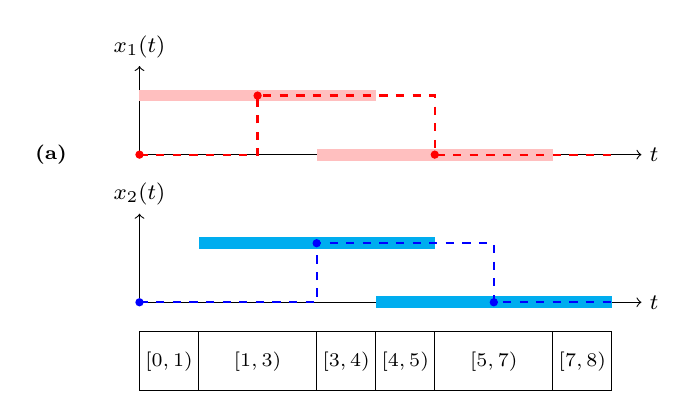
\begin{tikzpicture}[scale=0.75]
		\scriptsize
		\node at (-1.5,0) {\textbf{(a)}};
		\footnotesize 
		% Plot for x1(t)
		\begin{scope}
			% Axes
			\draw[->] (0,0) -- (8.5,0) node[right] {$t$};
			\draw[->] (0,0) -- (0,1.5) node[above] {$x_1(t)$};
			
			% Red shaded areas
			\fill[pink] (0,1.1) rectangle (4,0.9);
			\fill[pink] (3,0.1) rectangle (7,-0.1);
			
			% Red dashed lines
			\draw[red, thick, dashed] (0,0) -- (2,0) -- (2,1) -- (5,1) -- (5,0) -- (8,0);
			
			% Red dots
			\fill[red] (0,0) circle (2pt);
			\fill[red] (2,1) circle (2pt);
			\fill[red] (5,0) circle (2pt);
		\end{scope}
		
		% Plot for x2(t)
		\begin{scope}[shift={(0,-2.5)}]
			% Axes
			\draw[->] (0,0) -- (8.5,0) node[right] {$t$};
			\draw[->] (0,0) -- (0,1.5) node[above] {$x_2(t)$};
			
			% Red shaded areas
			\fill[cyan] (1,1.1) rectangle (5,0.9);
			\fill[cyan] (4,0.1) rectangle (8,-0.1);
			
			% Red dashed lines
			\draw[blue, thick, dashed] (0,0) -- (3,0) -- (3,1) -- (6,1) -- (6,0) -- (8,0);
			
			% Red dots
			\fill[blue] (0,0) circle (2pt);
			\fill[blue] (3,1) circle (2pt);
			\fill[blue] (6,0) circle (2pt);
		\end{scope}
		
		% GS boxes
		\begin{scope}[shift={(0,-4)}]
			\draw (0,0) rectangle (1,1);
			\node at (0.5,0.5) {{\scriptsize $[0,1)$}};
			\draw (1,0) rectangle (3,1);
			\node at (2,0.5) {{\scriptsize $[1,3)$}};
			\draw (3,0) rectangle (4,1);
			\node at (3.5,0.5) {{\scriptsize $[3,4)$}};
			\draw (4,0) rectangle (5,1);
			\node at (4.5,0.5) {{\scriptsize $[4,5)$}};
			\draw (5,0) rectangle (7,1);
			\node at (6,0.5) {{\scriptsize $[5,7)$}};
			\draw (7,0) rectangle (8,1);
			\node at (7.5,0.5) {{\scriptsize $[7,8)$}};
		\end{scope}
	\end{tikzpicture}
	\end{subfigure}
	\hspace{2em}
	\begin{subfigure}[c]{.45\textwidth}
		\centering
			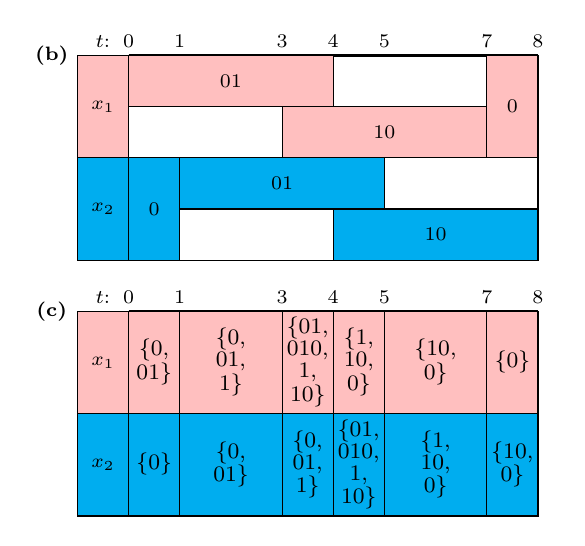
\begin{tikzpicture}[scale=0.65]
			\scriptsize
			% Part (a)
			\node at (-1.5,0) {\textbf{(b)}};
			\draw[thick] (0,0) -- (8,0);
			\foreach \x in {0,1,3,4,5,7,8}
			\draw (\x,0) node[above] {\x};
			\draw (-0.5,0) node[above] {$t$:};
			
			\draw[fill=pink] (-1,-2) rectangle (0,0) node[midway] {$x_1$};
			\draw[fill=pink] (0,-1) rectangle (4,0) node[midway] {$01$};
			\draw[fill=pink] (3,-2) rectangle (7,-1) node[midway] {$10$};
			\draw[fill=pink] (7,-2) rectangle (8,0) node[midway] {$0$};
			
			\draw[fill=cyan] (-1,-4) rectangle (0,-2) node[midway] {$x_2$};
			\draw[fill=cyan] (0,-4) rectangle (1,-2) node[midway] {$0$};
			\draw[fill=cyan] (1,-3) rectangle (5,-2) node[midway] {$01$};
			\draw[fill=cyan] (4,-4) rectangle (8,-3) node[midway] {$10$};
			
			\draw (0,-4) -- (8,-4);
			\draw (8,-4) -- (8,0);
			
			% Part (b)
			\node at (-1.5,-5) {\textbf{(c)}};
			\draw[thick] (0,-5) -- (8,-5);
			\foreach \x in {0,1,3,4,5,7,8}
			\draw (\x,-5) node[above] {\x};
			\draw (-0.5,-5) node[above] {$t$:};
			
			\draw[fill=pink] (-1,-7) rectangle (0,-5) node[midway] {$x_1$};
			\draw[fill=pink] (0,-7) rectangle (1,-5) node[midway] { \fontsize{8}{8}\selectfont \begin{tabular}{c}\{0,\\ 01\}\\\end{tabular}};
			\draw[fill=pink] (1,-7) rectangle (3,-5) node[midway] {\fontsize{8}{8}\selectfont\begin{tabular}{c}\{0,\\ 01,\\ 1\}\\\end{tabular}};
			\draw[fill=pink] (3,-7) rectangle (4,-5) node[midway] {\fontsize{8}{8}\selectfont{\begin{tabular}{c}\{01,\\ 010,\\ 1,\\ 10\}\\\end{tabular}}};
			\draw[fill=pink] (4,-7) rectangle (5,-5) node[midway] {\fontsize{8}{8}\selectfont\begin{tabular}{c}\{1,\\ 10,\\ 0\}\\\end{tabular}};
			\draw[fill=pink] (5,-7) rectangle (7,-5) node[midway] {{\fontsize{8}{8}\selectfont\begin{tabular}{c}\{10,\\ 0\}\\\end{tabular}}};
			\draw[fill=pink] (7,-7) rectangle (8,-5) node[midway] {{\fontsize{8}{8}\selectfont\begin{tabular}{c}\{0\}\\\end{tabular}}};
			
			\draw[fill=cyan] (-1,-9) rectangle (0,-7) node[midway] {$x_2$};
			\draw[fill=cyan] (0,-9) rectangle (1,-7) node[midway] {{\fontsize{8}{8}\selectfont\begin{tabular}{c}\{0\}\\\end{tabular}}};
			\draw[fill=cyan] (1,-9) rectangle (3,-7) node[midway] {\fontsize{8}{8}\selectfont\begin{tabular}{c}\{0,\\ 01\}\\\end{tabular}};
			\draw[fill=cyan] (3,-9) rectangle (4,-7) node[midway] {\fontsize{8}{8}\selectfont\begin{tabular}{c}\{0,\\ 01,\\ 1\}\\\end{tabular}};
			\draw[fill=cyan] (4,-9) rectangle (5,-7) node[midway] {\fontsize{8}{8}\selectfont{\begin{tabular}{c}\{01,\\ 010,\\ 1,\\ 10\}\\\end{tabular}}};
			\draw[fill=cyan] (5,-9) rectangle (7,-7) node[midway] {\fontsize{8}{8}\selectfont\begin{tabular}{c}\{1,\\ 10,\\ 0\}\\\end{tabular}};
			\draw[fill=cyan] (7,-9) rectangle (8,-7) node[midway] {{\fontsize{8}{8}\selectfont\begin{tabular}{c}\{10,\\ 0\}\\\end{tabular}}};
		\end{tikzpicture}
	\end{subfigure}
	\vspace{1ex}	
	\caption{\textbf{(a)} A distributed signal $(S,{\hb})$ with $x_1$ (top, red) and $x_2$ (bottom, blue) whose edges are marked with solid balls and their uncertainty regions are given as semi-transparent boxes around the edges. The resulting canonical segmentation $G_S$ is shown below the graphical representation of the signals. \textbf{(b)} The uncertainty regions of $(S,{\hb})$ and the corresponding value expressions. \textbf{(c)} The tabular representation of the function $\gamma$ for $(S,{\hb})$, e.g., \(\gamma(x_1, [3,4)) = (\sfx(01) \cdot \pfx(10)) \setminus \{\epsilon\} = \{ 01, 010, 1, 10\}\).\label{fig:csve}}
%	\vspace{1em}
\end{figure*}


\paragraph*{Value Expressions.}
Consider a Boolean signal \( x \) with a rising edge within an uncertainty region of \((t_1, t_2)\).
As mentioned, the monitor only knows that \( x \) changes from 0 to 1 in this interval.
This knowledge is represented as a finite word \( v = 01 \) over the alphabet \(\Sigma = \{0,1\}\).
This representation, called a \emph{value expression}, encodes the uncertain behavior of an observed signal relative to the monitor.
Formally, a value expression is an element of \(\Sigma^*\), where \(\Sigma\) is the finite alphabet of signal values.
Given a signal \( x \) and an edge \((t, x(t))\), the value expression corresponding to the uncertainty region \((\theta_{\text{lo}}(x,t), \theta_{\text{hi}}(x,t))\) is \( v_{x,t} = v_- \cdot v_+ \), where \( v_- = \lim_{s \to t^-} x(s) \) and \( v_+ = \lim_{s \to t^+} x(s) \).
We omit the concatenation symbol \(\cdot\) when the letters are clear from context.
This definition is general because finite-length piecewise-constant real-valued signals will only have a finite number of values, making \(\Sigma\) finite.

Notice that (i) uncertainty regions may overlap, and (ii) the canonical segmentation may split an uncertainty region into multiple segments.
Consider a signal $x$ with a rising edge in $(1,5)$ and a falling edge in $(4,8)$.
The corresponding value expressions are respectively $v_1 = 01$ and $v_2 = 10$.
Notice that the behavior of $x$ in the interval $[1,4)$ can be expressed as $\pfx(v_1)$, encoding whether the rising edge has happened yet.
Similarly, the behavior in $[4,5)$ is given by $\sfx(v_1) \cdot \pfx(v_2)$, which captures whether the edges occur in this interval (thanks to prefixing and suffixing) and the fact that the rising edge happens before the falling edge (thanks to concatenation).

%\begin{wrapfigure}{r}{0.5\textwidth}
%	%	\vspace{-2em}
%	
%
%\end{wrapfigure}

Formally, given a distributed signal $(S,{\hb})$, we define a function $\gamma : S \times G_S \to 2^{\Sigma^*}$ that maps each signal and segment of the canonical segmentation to a set of value expressions, capturing the signal's potential behaviors in the given segment.
Let $x$ be a signal in $S$, and let $R_1, \ldots, R_m$ be its uncertainty regions where $R_i = (t_i, t_i')$ and the corresponding value expression is $v_i$ for all $1 \leq i \leq m$.
Now, let $I \in G_S$ be a segment with $I = [s, s')$ and for each $1 \leq i \leq m$ define the set $V_i$ of value expressions capturing how $I$ relates with $R_i$ in \cref{eq:valexprset}.
%
\begin{figure}
%	\small
%	\vspace{-1em}
	\begin{equation} \label{eq:valexprset}
		V_i = 
		\begin{cases}
			\{v_i\} & \text{if } t_i = s \land s' = t_i' \\
			\pfx(v_i) & \text{if } t_i = s \land s' < t_i' \\
			\sfx(v_i) & \text{if } t_i > s \land s' = t_i' \\
			\infx(v_i) & \text{if } t_i > s \land s' < t_i' \\
			\{\epsilon\} & \text{otherwise}
		\end{cases}
	\end{equation}
%	\vspace{-2em}
\end{figure}
%\normalsize
The last case happens only when \( I \cap R_i \) is empty.
We define \(\gamma\) as follows:
%%\vspace{-1em}
\[ \gamma(x,I) = \destutter(V_1 \cdot V_2 \cdot \ldots \cdot V_m) \setminus \{\epsilon\} \]
%%\vspace{-1em}
Observe that \(\gamma(x,I)\) contains all the potential behaviors of \( x \) in segment \( I \) by construction.
However, it is potentially overapproximate because the sets \( V_1, \ldots, V_m \) contain redundancy by definition, and the concatenation does not ensure that an edge is considered exactly once -- see \cref{fig:csve}b and \cref{fig:csve}c.
%We demonstrate this in \cref{fig:csve}b and \cref{fig:csve}c.

%\begin{example} \label{ex:valexpr}
%	Recall the distributed signal \((S, {\hb})\) in \cref{fig:canonseg}.
%	In \cref{fig:valexpr}a, we show the value expressions corresponding to its uncertainty regions.
%	For example, the falling edge of \(x_1\) has an uncertainty region of \((3,7)\), represented by the value expression \(10\). 
%	In \cref{fig:valexpr}b, we give the function \(\gamma\) for \((S, {\hb})\).
%	For example, \(\gamma(x_1, [3,4)) = (\sfx(01) \cdot \pfx(10)) \setminus \{\epsilon\} = \{ 01, 010, 1, 10\}\), and \(\gamma(x_2, [0,1)) = \{0\}\).
%\end{example}




\paragraph*{Overapproximation of $\tr$.}
Consider a distributed signal $(S,{\hb})$ of $n$ signals, and let $G_S$ be its canonical segmentation.
We describe how the function $\gamma$ defines a set $\tr^+(S,{\hb})$ of synchronous traces that overapproximates the set $\tr(S,{\hb})$.
%
%Let $x : [0,d) \to \B$ be a signal.
%Consider the set $N_x$ of signals such that each $x' \in X$ is obtained from $x$ by shifting its edges within their uncertainty regions while preserving their relative order.
%Formally, we let $E = \{ (t_1, x(t_1)), \ldots, (t_m, x(t_m)) \}$ be the set of edges of $x$ with $t_i < t_{i+1}$ for all $1 \leq i < m$, let $R_1, \ldots, R_m$ be the corresponding uncertainty regions, and define $N_x$ as follows: 
%$$ N_x = \{x' : [0,d) \to \B \st x'(0) = x(0) \land \forall 1 \leq i \leq m : t_i' \in R_i \land x'(t_i') = x(t_i) \} $$ where $E' = \{ (t_1', x'(t_1')), \ldots, (t_m', x'(t_m')) \}$ is the set of edges of $x'$ with $t_i' < t_{i+1}'$ for all $1 \leq i < m$.
%For example, ...
%
%Now, 
%Let $x \in S$ and $x'$ be two signals with the same temporal domain, and let $I = [s, s')$ be a segment in $G_S$.
%Let $(t_1, x'(t_1)), \ldots, (t_\ell, x'(t_\ell))$ be the edges of $x'$ in segment $I$ with $t_i < t_{i+1}$ for all $1 \leq i < \ell$.
%The signals $x$ and $x'$ are \emph{consistent in $I$} iff $x(s) = x'(s)$ and the value expression $x'(s) \cdot x'(t_1) \cdot \ldots \cdot x'(t_\ell)$ belongs to $\gamma(x,I)$.
%Moreover, $x$ and $x'$ are \emph{consistent} iff they are consistent in $I$ for all $I \in G_S$.
%Now, let $S = (x_1, \ldots, x_n)$ and define the \emph{canonical overapproximation} of $(S,{\hb})$ as follows:
%$$ \tr^+(S,{\hb}) = \{ (x_1', \ldots, x_n') \st \text{$x_i$ and $x_i'$ are consistent for all $1 \leq i \leq n$}\} $$
%
Consider $x \in S$, and let $x'$ be a signal with the same temporal domain, and let $I = [s, s')$ be a segment in $G_S$.
Let $(t_1, x'(t_1)), \ldots, (t_\ell, x'(t_\ell))$ be the edges of $x'$ in segment $I$ with $t_i < t_{i+1}$ for all $1 \leq i < \ell$.
The signal $x'$ is \emph{$I$-consistent with $x$} iff the value expression $x'(s) \cdot x'(t_1) \cdot \ldots \cdot x'(t_\ell)$ belongs to $\gamma(x,I)$.
Moreover, $x'$ is \emph{consistent with $x$} iff it is $I$-consistent with $x$ for all $I \in G_S$.
Now, let $S = (x_1, \ldots, x_n)$ and define $\tr^+(S,{\hb})$ as follows:
%\vspace{-0.5em}
\begin{align*}
	\tr^+(S,{\hb}) = \{ (x_1', \ldots, x_n') \st \text{$x_i'$ is consistent with}&\\
	\text{$x_i$ for all $1 \leq i \leq n$}&\} 
\end{align*}
%%\vspace{-1em}


\begin{example} \label{ex:overapx}
	Recall \((S, {\hb})\) and its \(\gamma\) function from \cref{fig:csve}.
	Consider the synchronous trace \(w \in \tr(S, {\hb})\) where the rising edges of both signals occur at time 3 and the falling edges at time 5.
	Such a signal \( w \) would be included in \(\tr^+(S,{\hb})\) since for each \(i \in \{1,2\}\), the value expression 1 is contained in \(\gamma(x_i, [3,4))\) and \(\gamma(x_i, [4,5))\), while 0 is contained in the remaining sets \(\gamma\) maps \(x_i\) to.
	Now, consider a synchronous trace \((x_1', x_2')\) where both signals are initially 0, have rising edges at time 2 and 3.5, and falling edges at time 3 and 5.
	This trace does not belong to \(\tr(S, {\hb})\) since \(x_1'\) and \(x_2'\) have more edges than \(x_1\) and \(x_2\).
	However, it belongs to \(\tr^+(S,{\hb})\) since \(x_1'\) and \(x_2'\) are consistent with \(x_1\) and \(x_2\).
	Specifically, for each \(i \in \{1,2\}\), the value expression \(01\) is contained in \(\gamma(x_i, [1,3))\) and \(\gamma(x_i, [3,4))\), the expression \(1\) is contained in \(\gamma(x_i, [4,5))\), and 0 is contained in the remaining sets \(\gamma\) maps \(x_i\) to.
\end{example}

Notice that any trace in $\tr(S,\hb)$ can be seen as an $\varepsilon$-retiming of the original signal.
Putting it all together, we finally prove that $\tr^+$ overapproximates $\tr$.

\begin{lemma} \label{cl:trsound}
	For every distributed signal $(S,{\hb})$, we have $\tr(S,{\hb}) \subseteq \tr^+(S,{\hb})$.
\end{lemma}
\begin{proof}[\normalsize Proof.]
	\normalsize
	Let $(S,{\hb})$ be a distributed signal where $S = (x_1, \ldots, x_n)$.
	Let $w = (y_1, \ldots, y_n) \in \tr(S,{\hb})$ be a trace.
	We want to show that $w \in \tr^+(S,{\hb})$.
	First, let us recall the definition of $\tr^+$.
	\begin{align*}
		\tr^+(S,{\hb}) = \{ (x_1', \ldots, x_n') \st \text{$x_i'$ is consistent with}&\\
		\text{$x_i$ for all $1 \leq i \leq n$}&\} 
	\end{align*}
	
	Let $1 \leq i \leq n$ be arbitrary.
	To show that $y_i$ is consistent with $x_i$, we need to show that $y_i$ is $I$-consistent with $x_i$ for all $I \in G_S$.
	Let $I = [t_0, s)$ be an arbitrary segment in $G_S$, let $(t_1, y_i(t_1)), \ldots, (t_\ell, y_i(t_\ell))$ be the edges of $y_i$ in segment $I$ with $t_j < t_{j+1}$ for all $1 \leq j < \ell$.
	To show that $y_i$ is $I$-consistent with $x_i$, we need to show that the expression $y_i(t_0) \cdot y_i(t_1) \cdot \ldots \cdot y_i(t_\ell)$ belongs to $\gamma(x_i,I)$.
	We sketch the proof idea below.
	
	Note that $w$ can be seen as a trace obtained through an $\varepsilon$-retiming of $S$ (\cite[Section 4.2]{MomtazAB23}).
	Then, the timestamp $t$ of any edge of $x_i$ is mapped to some clock value in the range $(\theta_{\text{lo}}(t), \theta_{\text{hi}}(t))$.
	In particular, $|t - c^{-1}_i(t)| < \varepsilon$ for all $t \in \{t_0, t_1, \ldots, t_\ell\}$, where $c^{-1}_i(t)$ is the local clock value of $x_i$ mapped to $t$.
	
	Since $y_i$ has $\ell$ edges in $I$, it holds that $x_i$ has at least $\ell$ edges in $(t_0 - \varepsilon, s + \varepsilon)$.
	Since $I$ is a segment in $G_S$, there are $\ell$ of these that are consecutive such that the intersection of their uncertainty regions contain $(t_0,s)$, i.e., $(t_0,s) \subseteq \bigcap_{1 \leq j \leq \ell} (\theta_{\text{lo}}(t_j'), \theta_{\text{hi}}(t_j'))$ where $t_j' = c^{-1}_i(t_j)$ is the corresponding timestamp in $x_i$ for all $0 \leq j \leq \ell$.
	In particular, note that $y_i(t_j) = x_i(t_j')$ for all $0 \leq j \leq \ell$.
	
	Now, notice that, by definition, $\gamma(x_i, I)$ takes into account every edge of $x_i$ whose uncertainty region has a nonempty intersection with $I$, and preserves their order.
	Let $V_j$ be the set of value expressions capturing how $I$ relates with the uncertainty intervals of the edge $(t_j', x_i(t_j'))$ for all $1 \leq j \leq \ell$ (as defined in \cref{eq:valexprset}).
	Then, $\destutter(\{x_i(t_0')\} \cdot V_1 \cdot \ldots \cdot V_\ell) \subseteq \gamma(x_i, I)$.
	One can verify that for all $1 \leq j \leq \ell$, either $x_i(t_j')$ or $x_i(t_{j-1}') \cdot x_i(t_j')$ belongs to $V_j$.
	This allows us to choose a value expression $v_j$ from each $V_j$ such that $\destutter(\{x_i(t_0')\} \cdot v_1 \cdot \ldots \cdot v_\ell) = x_i(t_0') \cdot x_i(t_1') \cdot \ldots \cdot x_i(t_\ell')$, which concludes the proof. 
	
	Note that if there are more edges of $x_i$ with a timestamp smaller than $t_0'$ or larger than $t_\ell'$ whose uncertainty intervals intersect with $I$, then the corresponding set of value expressions is obtained either by prefixing or suffixing.
	In either case, we can choose $\epsilon$ from these sets for concatenation with the remaining edges' value expressions and obtain the desired result.
\end{proof}
